% Lecture 1: The History of IT Ethics
% IT Ethics Course
% Brendan Shea, PhD - Rochester Community and Technical College

\documentclass[aspectratio=169]{beamer}

% Theme and styling
\usetheme{Madrid}
\usecolortheme{default}
\setbeamertemplate{navigation symbols}{}
\setbeamertemplate{footline}[frame number]

% Packages
\usepackage{tikz}
\usetikzlibrary{shapes,arrows,positioning,calc,fit,backgrounds}
\usepackage{booktabs}
\usepackage{array}
\usepackage{graphicx}
% Custom icons (text-based alternatives)
\newcommand{\faQuoteLeft}{\textbf{``}}
\newcommand{\faBalanceScale}{$\triangleright$}
\newcommand{\faComments}{\textbf{?}}
\newcommand{\faLightbulb}{$\star$}
\newcommand{\faThumbsUp}{\textbf{+}}
\newcommand{\faThumbsDown}{\textbf{--}}

% Custom colors
\definecolor{primaryblue}{RGB}{0,73,135}
\definecolor{accentgold}{RGB}{198,146,20}
\definecolor{darkgray}{RGB}{64,64,64}
\definecolor{lightgray}{RGB}{240,240,240}
\definecolor{quotegreen}{RGB}{34,139,34}

% Set theme colors
\setbeamercolor{structure}{fg=primaryblue}
\setbeamercolor{title}{fg=white,bg=primaryblue}
\setbeamercolor{frametitle}{fg=white,bg=primaryblue}
\setbeamercolor{block title}{fg=white,bg=primaryblue}
\setbeamercolor{block body}{bg=lightgray}
\setbeamercolor{block title alerted}{fg=white,bg=red!70!black}
\setbeamercolor{block body alerted}{bg=red!10}
\setbeamercolor{block title example}{fg=white,bg=quotegreen}
\setbeamercolor{block body example}{bg=green!5}

% Custom environments for consistent formatting

% Quote environment
\newenvironment{quoteslide}[2]{%
  \begin{exampleblock}{\faQuoteLeft\hspace{0.5em}#1}
  \small
  \textit{``#2''}
}{%
  \end{exampleblock}
}

% Argument environment
\newenvironment{argument}{%
  \begin{block}{\faBalanceScale\hspace{0.5em}Argument in Standard Form}
  \begin{enumerate}
}{%
  \end{enumerate}
  \end{block}
}

% Discussion question environment
\newcommand{\discussion}[1]{%
  \begin{alertblock}{\faComments\hspace{0.5em}Discussion Question}
  #1
  \end{alertblock}
}

% Title information
\title[History of IT Ethics]{Lecture 1: The History of IT Ethics}
\subtitle{IT Ethics}
\author{Brendan Shea, PhD}
\institute{Rochester Community and Technical College}
\date{}

\begin{document}

% ====================
% TITLE SLIDE
% ====================
\begin{frame}
\titlepage
\end{frame}

% ====================
% INTRODUCTION (Slides 2-4)
% ====================

\begin{frame}{What is Information Technology?}
\textbf{Definition:} Technologies for \textbf{creating}, \textbf{storing}, \textbf{transmitting}, and \textbf{processing} information.

\vspace{0.5em}
\begin{block}{Key Insight}
Information technology is \textbf{ancient}---not just computers!
\end{block}

\vspace{0.3em}
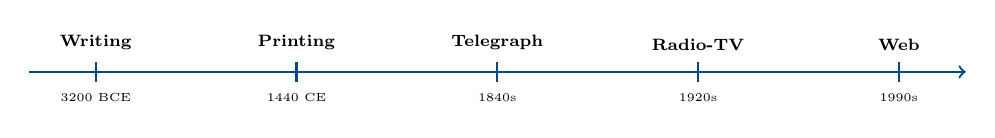
\begin{tikzpicture}[scale=0.85, transform shape]
  \draw[thick, ->, primaryblue] (0,0) -- (14,0);
  \foreach \x/\label/\year in {1/Writing/3200 BCE, 4/Printing/1440 CE, 7/Telegraph/1840s, 10/Radio-TV/1920s, 13/Web/1990s} {
    \draw[thick, primaryblue] (\x,0.15) -- (\x,-0.15);
    \node[above, font=\scriptsize\bfseries] at (\x,0.2) {\label};
    \node[below, font=\tiny] at (\x,-0.2) {\year};
  }
\end{tikzpicture}

\vspace{0.5em}
\discussion{What's the oldest information technology you can think of?}
\end{frame}

\begin{frame}{What is Normative Ethics?}
\textbf{Definition:} The branch of philosophy concerned with how we \textbf{ought} to act.

\vspace{0.5em}
\begin{block}{Three Branches of Ethics}
\begin{itemize}
  \item \textbf{Descriptive Ethics:} What people \textit{do} believe about right and wrong
  \item \textbf{Normative Ethics:} What people \textit{should} believe about right and wrong
  \item \textbf{Metaethics:} The nature of morality itself (e.g., Are moral facts real?)
\end{itemize}
\end{block}

\vspace{0.3em}
\begin{alertblock}{Key Insight}
Ethics is also \textbf{ancient}---as old as philosophy itself!
\end{alertblock}

\vspace{0.3em}
\discussion{When we say something is ``unethical,'' what do we mean?}
\end{frame}

\begin{frame}{The Five IT Revolutions}
\begin{block}{Roadmap for Today's Lecture}
We will examine five major information technology revolutions, each with its own debates, promises, and unforeseen consequences.
\end{block}

\vspace{0.3em}
\begin{table}
\centering
\small
\begin{tabular}{@{}clll@{}}
\toprule
\textbf{\#} & \textbf{Revolution} & \textbf{Approximate Date} & \textbf{Key Thinkers} \\
\midrule
1 & Writing & $\sim$3200 BCE & Socrates, Plato \\
2 & Printing Press & $\sim$1440 CE & Luther, Erasmus \\
3 & Distance Communication & $\sim$1840s & Mill, Marx \\
4 & Mass Media & $\sim$1920s & Orwell, Arendt \\
5 & The Web & $\sim$1990s & Current debates \\
\bottomrule
\end{tabular}
\end{table}

\vspace{0.3em}
\begin{exampleblock}{Central Theme}
Each revolution promised liberation---and each enabled new forms of control.
\end{exampleblock}
\end{frame}

% ====================
% REVOLUTION 1: WRITING (Slides 5-11)
% ====================

\begin{frame}{Revolution 1: A Brief History of Writing}
\begin{columns}
\begin{column}{0.55\textwidth}
\begin{block}{Key Developments}
\begin{itemize}
  \item \textbf{Cuneiform} in Mesopotamia ($\sim$3200 BCE)
  \item \textbf{Egyptian hieroglyphics} ($\sim$3100 BCE)
  \item \textbf{Phoenician alphabet} ($\sim$1050 BCE)
  \item \textbf{Greek alphabet} ($\sim$800 BCE)
\end{itemize}
\end{block}

\begin{alertblock}{Writing as Memory Technology}
Writing \textbf{externalizes} information---storing it outside the human mind for the first time.
\end{alertblock}
\end{column}

\begin{column}{0.42\textwidth}
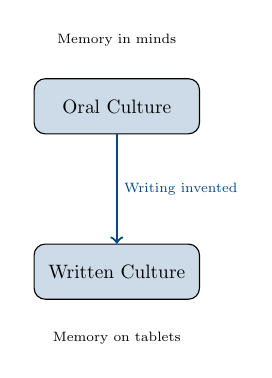
\begin{tikzpicture}[scale=0.7, transform shape]
  \node[draw, rounded corners, fill=primaryblue!20, minimum width=3cm, minimum height=1cm] (oral) at (0,3) {Oral Culture};
  \node[draw, rounded corners, fill=primaryblue!20, minimum width=3cm, minimum height=1cm] (written) at (0,0) {Written Culture};
  \draw[->, thick, primaryblue] (oral) -- (written) node[midway, right, font=\scriptsize] {Writing invented};
  \node[font=\scriptsize, text width=3cm, align=center] at (0,4.2) {Memory in minds};
  \node[font=\scriptsize, text width=3cm, align=center] at (0,-1.2) {Memory on tablets};
\end{tikzpicture}
\end{column}
\end{columns}

\vspace{0.3em}
\discussion{What might be \textbf{lost} when a culture shifts from oral tradition to written records?}
\end{frame}

\begin{frame}{Who Were Socrates and Plato?}
\begin{columns}
\begin{column}{0.48\textwidth}
\begin{block}{Socrates (c. 470--399 BCE)}
\begin{itemize}
  \item Athenian philosopher; wrote \textbf{nothing}
  \item Taught through \textbf{dialogue} and questioning
  \item The ``\textbf{Socratic method}'': Learn by examining your own beliefs
  \item Executed for ``corrupting the youth''
  \item We know him only through others' writings
\end{itemize}
\end{block}
\end{column}

\begin{column}{0.48\textwidth}
\begin{exampleblock}{Plato (c. 428--348 BCE)}
\begin{itemize}
  \item Socrates's most famous student
  \item Founded the \textbf{Academy} in Athens
  \item Wrote \textbf{dialogues} featuring Socrates
  \item Key works: \textit{Republic}, \textit{Phaedrus}, \textit{Apology}
  \item Preserved Socrates's ideas \textit{in writing}
\end{itemize}
\end{exampleblock}
\end{column}
\end{columns}

\vspace{0.5em}
\begin{alertblock}{The Central Irony}
Socrates distrusted writing---but we only know this \textbf{because Plato wrote it down}. Would Socrates have approved of Plato's project?
\end{alertblock}
\end{frame}

\begin{frame}{Socrates and Plato's Worries About Writing}
\begin{columns}
\begin{column}{0.6\textwidth}
\begin{block}{The Irony}
\textbf{Socrates} never wrote anything down---yet we know his views through \textbf{Plato's} written dialogues.
\end{block}

\vspace{0.3em}
\begin{exampleblock}{Plato's \textit{Phaedrus} (c. 370 BCE)}
Socrates tells the \textbf{myth of Theuth and Thamus}:
\begin{itemize}
  \item \textbf{Theuth}: Egyptian god who invents writing
  \item \textbf{Thamus}: King who must judge the invention
  \item Theuth claims writing will make people ``wiser''
  \item Thamus disagrees...
\end{itemize}
\end{exampleblock}
\end{column}

\begin{column}{0.38\textwidth}
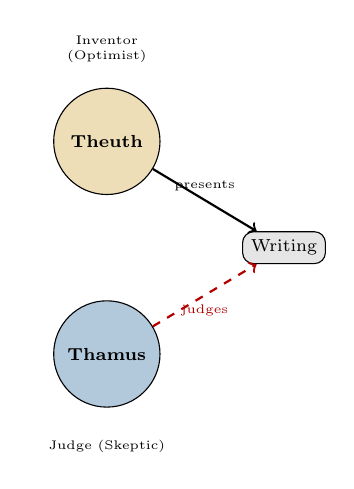
\begin{tikzpicture}[scale=0.9, transform shape]
  \node[draw, circle, fill=accentgold!30, minimum size=1.5cm, font=\scriptsize\bfseries] (theuth) at (0,2) {Theuth};
  \node[draw, circle, fill=primaryblue!30, minimum size=1.5cm, font=\scriptsize\bfseries] (thamus) at (0,-1) {Thamus};
  \node[draw, rectangle, rounded corners, fill=gray!20, font=\scriptsize] (writing) at (2.5,0.5) {Writing};
  \draw[->, thick] (theuth) -- (writing) node[midway, above, font=\tiny] {presents};
  \draw[->, thick, dashed, red!70!black] (thamus) -- (writing) node[midway, below, font=\tiny] {judges};
  \node[font=\tiny, text width=2cm, align=center] at (0,3.3) {Inventor (Optimist)};
  \node[font=\tiny, text width=2cm, align=center] at (0,-2.3) {Judge (Skeptic)};
\end{tikzpicture}
\end{column}
\end{columns}
\end{frame}

\begin{frame}{Quote: Plato's \textit{Phaedrus} on Writing}
\begin{exampleblock}{\faQuoteLeft\hspace{0.5em}Plato, \textit{Phaedrus}, 275a-b (Fowler trans.)}
\small
\textbf{Context:} King Thamus responds to Theuth's claim that writing will improve memory and wisdom:

\vspace{0.5em}
\textit{``For this invention will produce \textbf{forgetfulness} in the minds of those who learn to use it, because they will not practice their memory. Their trust in writing, produced by external characters which are no part of themselves, will discourage the use of their own memory within them.}

\vspace{0.3em}
\textit{You have invented an elixir not of \textbf{memory}, but of \textbf{reminding}; and you offer your pupils the \textbf{appearance of wisdom}, not true wisdom, for they will read many things without instruction and will therefore seem to know many things, when they are for the most part ignorant and hard to get along with, since they are not wise, but only \textbf{appear} wise.''}
\end{exampleblock}

\vspace{0.3em}
\begin{block}{\faLightbulb\hspace{0.5em}Key Distinctions}
\textbf{Memory} (internal) vs. \textbf{Reminding} (external) \quad|\quad \textbf{True wisdom} vs. \textbf{Appearance of wisdom}
\end{block}
\end{frame}

\begin{frame}{Socrates's Argument Against Writing}
\begin{argument}
  \item True knowledge requires \textbf{active engagement}, dialogue, and the ability to respond to questions.
  \item Writing \textbf{cannot respond} to questions or adapt to its audience.
  \item Writing therefore creates the \textbf{appearance of wisdom} without its reality.
  \item[\textbf{$\therefore$}] Writing is \textbf{inferior} to living discourse for producing genuine understanding.
\end{argument}

\vspace{0.5em}
\discussion{Is this argument \textbf{sound}? What might Socrates be missing?}

\vspace{0.3em}
\begin{alertblock}{The Paradox}
We only know Socrates's anti-writing argument \textit{because Plato wrote it down}!
\end{alertblock}
\end{frame}

\begin{frame}{Social Consequences of Writing}
\begin{columns}
\begin{column}{0.48\textwidth}
\begin{block}{\faThumbsUp\hspace{0.3em}Benefits}
\begin{itemize}
  \item \textbf{Law codes} (Hammurabi, Torah)
  \item \textbf{Historical records} and memory
  \item \textbf{Literature} and poetry
  \item \textbf{Religious texts} preserved
  \item \textbf{Scholarship} across generations
  \item \textbf{Contracts} and commerce
\end{itemize}
\end{block}
\end{column}

\begin{column}{0.48\textwidth}
\begin{alertblock}{\faThumbsDown\hspace{0.3em}Harms}
\begin{itemize}
  \item \textbf{Imperial administration} and control
  \item \textbf{Social stratification}: literate elite vs. illiterate masses
  \item \textbf{Loss of oral traditions}
  \item \textbf{Bureaucratic power} over individuals
  \item \textbf{Propaganda} becomes possible
\end{itemize}
\end{alertblock}
\end{column}
\end{columns}

\vspace{0.5em}
\begin{exampleblock}{Key Insight}
The same technology that enables law and literature also enables empire and control.
\end{exampleblock}
\end{frame}

\begin{frame}{The Pattern Emerges}
\begin{center}
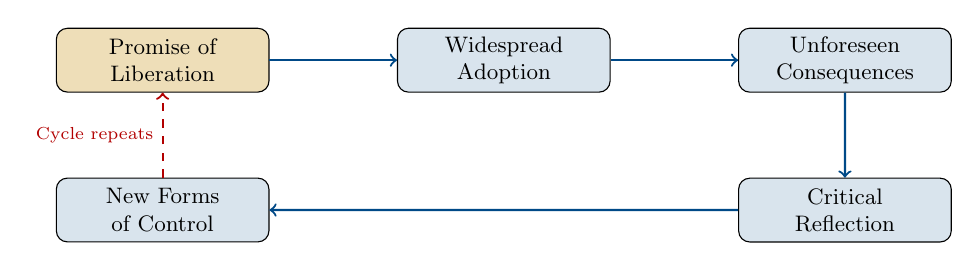
\begin{tikzpicture}[scale=0.9, transform shape, 
    node distance=1.8cm,
    box/.style={draw, rounded corners, fill=primaryblue!15, minimum width=3cm, minimum height=0.9cm, align=center, font=\small}]
  
  \node[box, fill=accentgold!30] (promise) {Promise of\\Liberation};
  \node[box, right=of promise] (adoption) {Widespread\\Adoption};
  \node[box, right=of adoption] (consequences) {Unforeseen\\Consequences};
  \node[box, below=1.2cm of consequences] (reflection) {Critical\\Reflection};
  \node[box, below=1.2cm of promise] (control) {New Forms\\of Control};
  
  \draw[->, thick, primaryblue] (promise) -- (adoption);
  \draw[->, thick, primaryblue] (adoption) -- (consequences);
  \draw[->, thick, primaryblue] (consequences) -- (reflection);
  \draw[->, thick, primaryblue] (reflection) -- (control);
  \draw[->, thick, dashed, red!70!black] (control) -- (promise) node[midway, left, font=\scriptsize] {Cycle repeats};
\end{tikzpicture}
\end{center}

\vspace{0.3em}
\begin{block}{Recurring Themes}
\begin{itemize}
  \item New IT \textbf{promises liberation} and democratization
  \item Critics warn of \textbf{unintended consequences}
  \item \textbf{Both} turn out to be partially right
  \item The technology \textbf{serves whoever controls it}
\end{itemize}
\end{block}
\end{frame}

% ====================
% REVOLUTION 2: PRINTING PRESS (Slides 12-18)
% ====================

\begin{frame}{Revolution 2: A Brief History of Printing}
\begin{block}{Key Developments}
\begin{itemize}
  \item \textbf{Chinese woodblock printing} (9th century CE)
  \item \textbf{Gutenberg's movable type} ($\sim$1440, Mainz, Germany)
  \item \textbf{Rapid spread} across Europe: Venice, Paris, London
  \item \textbf{Economics}: Cost of a book drops dramatically
\end{itemize}
\end{block}

\vspace{0.3em}
\begin{exampleblock}{Scale of Change}
Before printing: A single book might cost as much as a \textbf{house}.\\
After printing: Books become affordable to the middle class.
\end{exampleblock}

\vspace{0.3em}
\discussion{The printing press made it possible to spread ideas rapidly and widely. Can you think of situations where that might be \textbf{dangerous}?}
\end{frame}

\begin{frame}{Johannes Gutenberg and the Printing Press}
\begin{columns}
\begin{column}{0.52\textwidth}
\begin{block}{Johannes Gutenberg (c. 1400--1468)}
\begin{itemize}
  \item German blacksmith and inventor
  \item Developed \textbf{movable type} ($\sim$1440)
  \item Key innovations: metal alloy type, oil-based ink, wooden press adapted from wine presses
  \item \textbf{Gutenberg Bible} (1455): First major book printed in Europe
  \item Died in relative obscurity
\end{itemize}
\end{block}
\end{column}

\begin{column}{0.45\textwidth}
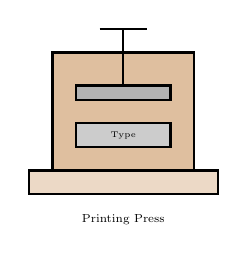
\begin{tikzpicture}[scale=0.6, transform shape]
  % Simple printing press diagram
  \draw[thick, fill=brown!30] (0,0) rectangle (4,0.5); % base
  \draw[thick, fill=brown!50] (0.5,0.5) rectangle (3.5,3); % frame
  \draw[thick, fill=gray!40] (1,1) rectangle (3,1.5); % type bed
  \node[font=\tiny] at (2,1.25) {Type};
  \draw[thick, fill=gray!60] (1,2) rectangle (3,2.3); % platen
  \draw[thick] (2,2.3) -- (2,3.5); % screw
  \draw[thick] (1.5,3.5) -- (2.5,3.5); % handle
  \node[font=\scriptsize, below] at (2,-0.3) {Printing Press};
\end{tikzpicture}

\vspace{0.3em}
\begin{exampleblock}{The Impact}
By 1500: $\sim$20 million books printed in Europe (vs. a few thousand manuscripts before)
\end{exampleblock}
\end{column}
\end{columns}
\end{frame}

\begin{frame}{Luther vs. Erasmus: Revolution vs. Reform}
\begin{columns}
\begin{column}{0.55\textwidth}
\begin{block}{Martin Luther (1483--1546)}
\begin{itemize}
  \item Used the press to spread \textbf{radical reformation}
  \item 95 Theses (1517) spread across Germany in \textbf{weeks}
  \item German Bible becomes a \textbf{bestseller}
  \item Saw printing as \textbf{providential}
\end{itemize}
\end{block}

\begin{alertblock}{Erasmus of Rotterdam (1466--1536)}
\begin{itemize}
  \item Advocated \textbf{gradual reform} through scholarship
  \item Worried about \textbf{unlearned masses} reading complex texts
  \item Same technology, \textbf{different vision} of change
\end{itemize}
\end{alertblock}
\end{column}

\begin{column}{0.42\textwidth}
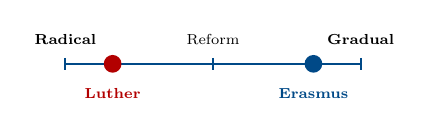
\begin{tikzpicture}[scale=0.75, transform shape]
  \draw[thick, primaryblue] (0,0) -- (5,0);
  \draw[thick, primaryblue] (0,0.1) -- (0,-0.1);
  \draw[thick, primaryblue] (5,0.1) -- (5,-0.1);
  \draw[thick, primaryblue] (2.5,0.1) -- (2.5,-0.1);
  \node[above, font=\scriptsize\bfseries] at (0,0.2) {Radical};
  \node[above, font=\scriptsize\bfseries] at (5,0.2) {Gradual};
  \node[above, font=\scriptsize] at (2.5,0.2) {Reform};
  \node[below, font=\scriptsize\bfseries, text=red!70!black] at (0.8,-0.3) {Luther};
  \node[below, font=\scriptsize\bfseries, text=primaryblue] at (4.2,-0.3) {Erasmus};
  \fill[red!70!black] (0.8,0) circle (0.15);
  \fill[primaryblue] (4.2,0) circle (0.15);
\end{tikzpicture}

\vspace{1em}
\begin{exampleblock}{Key Question}
Same technology, different visions---who gets to decide how it's used?
\end{exampleblock}
\end{column}
\end{columns}
\end{frame}

\begin{frame}{Quote: Martin Luther on Printing}
\begin{exampleblock}{\faQuoteLeft\hspace{0.5em}Martin Luther on the Printing Press}
\small
\textbf{Context:} Luther was among the first to recognize printing's transformative potential. His 95 Theses (1517) spread across Germany in weeks. His German Bible became a bestseller. For Luther, this was providential---God's plan unfolding through technology.

\vspace{0.5em}
\textit{``The art of book printing is the \textbf{last and greatest gift} because it is through this that the question of the true religion will become known to the \textbf{entire world}---to the very ends of the earth and in all languages---in accordance with God's will. It is the \textbf{inextinguishable flame} of the world.''}

\vspace{0.3em}
\hfill---Martin Luther, as quoted in Otto Clemen, \textit{Die lutherische Reformation und der Buchdruck}
\end{exampleblock}

\vspace{0.3em}
\begin{block}{\faLightbulb\hspace{0.5em}The Tension}
Luther sees printing as \textbf{divinely ordained} for spreading truth. But what happens when others use the same press to spread what Luther would call \textbf{error}? Luther himself wrote a highly polemical "On the Jews and Their Lies" later in life, which was cited by Nazis to justify anti-Semitic policies.
\end{block}
\end{frame}

\begin{frame}{The Erasmian Counterargument}
\begin{argument}
  \item Rapid, uncontrolled spread of ideas leads to \textbf{misunderstanding and conflict}.
  \item Complex theological and philosophical texts require \textbf{learned interpretation}.
  \item The printing press enables \textbf{unlearned masses} to access such texts without guidance.
  \item[\textbf{$\therefore$}] Printing requires \textbf{responsible gatekeeping} and scholarly mediation.
\end{argument}

\vspace{0.5em}
\discussion{Who gets to be the \textbf{gatekeeper}? And who decides?}

\vspace{0.3em}
\begin{alertblock}{The Dilemma}
Both Luther and Erasmus have a point---but their positions are in tension. Is there a middle ground?
\end{alertblock}
\end{frame}

\begin{frame}{Social Consequences of Printing: The Good}
\begin{block}{\faThumbsUp\hspace{0.3em}Benefits of the Printing Revolution}
\begin{itemize}
  \item \textbf{Scientific Revolution}: Sharing of data, replication of experiments, cumulative knowledge
  \item \textbf{Mass literacy campaigns}: Reading becomes a widespread skill
  \item \textbf{Vernacular literature}: National languages emerge (Dante, Shakespeare, Luther's German)
  \item \textbf{Religious diversity}: Individual conscience, Protestant Reformation
  \item \textbf{Philosophical treatises} widely available (Enlightenment becomes possible)
  \item \textbf{Standardization}: Spelling, grammar, shared reference texts
\end{itemize}
\end{block}

\vspace{0.3em}
\begin{exampleblock}{The Promise Fulfilled}
Printing \textit{did} democratize knowledge and enable new forms of intellectual community.
\end{exampleblock}
\end{frame}

\begin{frame}{Social Consequences of Printing: The Bad}
\begin{alertblock}{\faThumbsDown\hspace{0.3em}Dark Side of the Printing Revolution}
\begin{itemize}
  \item \textbf{\textit{Malleus Maleficarum}} (1487): The witch-hunting manual becomes a bestseller
  \item \textbf{Anti-Semitic pamphlets}: Pogroms spread with printed propaganda (e.g., Luther's later writings)
  \item \textbf{Religious wars}: Thirty Years' War (1618--1648) kills $\sim$8 million
  \item \textbf{Propaganda and polarization}: Pamphleteering as political warfare
  \item \textbf{State power consolidated}: Printed laws, surveillance records, bureaucracy
\end{itemize}
\end{alertblock}

\vspace{0.3em}
\discussion{Does the printing press bear \textbf{responsibility} for the witch trials? Or is it just a tool?}

\vspace{0.3em}
\begin{block}{The Pattern Repeats}
The same technology that enables the Scientific Revolution also enables mass propaganda.
\end{block}
\end{frame}

\begin{frame}{The Pattern Repeats}
\begin{center}
\begin{tabular}{@{}p{3cm}p{5cm}p{5cm}@{}}
\toprule
& \textbf{Writing} & \textbf{Printing} \\
\midrule
\textbf{Promise} & Preserve knowledge & Democratize knowledge \\
\textbf{Optimist} & Theuth & Luther \\
\textbf{Pessimist} & Thamus/Socrates & Erasmus \\
\textbf{Benefits} & Law, literature, scholarship & Science, literacy, Enlightenment \\
\textbf{Harms} & Empire, bureaucracy & Religious war, propaganda \\
\textbf{Key Question} & Who controls access? & Who controls the press? \\
\bottomrule
\end{tabular}
\end{center}

\vspace{0.5em}
\begin{exampleblock}{Emerging Insight}
The technology \textbf{amplifies human intentions}---both good and bad. The question is always: \textbf{Who controls it, and for what ends?}
\end{exampleblock}
\end{frame}

% ====================
% REVOLUTION 3: DISTANCE COMMUNICATION (Slides 19-24)
% ====================

\begin{frame}{Revolution 3: The Technologies of the Long 19th Century}
\begin{block}{Key Innovations}
\begin{itemize}
  \item \textbf{Telegraph} (1840s)---``The Victorian Internet''
  \item \textbf{Telephone} (1876)---Voice across distance
  \item \textbf{Undersea cables}---Connecting continents
  \item \textbf{Postal systems and railroads}---Physical distribution at scale
  \item \textbf{Photography and recorded sound}---New forms of documentation
\end{itemize}
\end{block}

\vspace{0.3em}
\begin{exampleblock}{The Optimistic 19th Century}
Many believed these technologies would \textbf{unite humanity} and \textbf{end war} through better communication.
\end{exampleblock}

\vspace{0.3em}
\discussion{The telegraph promised to unite humanity and end war. Why might people \textbf{keep believing this} about new technologies?}
\end{frame}

\begin{frame}{The Telegraph: ``The Victorian Internet''}
\begin{columns}
\begin{column}{0.55\textwidth}
\begin{block}{How It Worked}
\begin{itemize}
  \item \textbf{Morse code}: Letters encoded as electrical pulses (dots and dashes)
  \item Messages sent through \textbf{copper wires}
  \item Required \textbf{trained operators} at each end
  \item First message (1844): ``What hath God wrought!''
\end{itemize}
\end{block}

\begin{exampleblock}{Key Milestones}
\begin{itemize}
  \item \textbf{1858}: First transatlantic cable (failed after weeks)
  \item \textbf{1866}: Permanent transatlantic connection
  \item \textbf{1870s}: Global network connects continents
\end{itemize}
\end{exampleblock}
\end{column}

\begin{column}{0.42\textwidth}
\begin{alertblock}{The Hype}
\small
\textit{``The telegraph will unite all nations... Wars will cease to exist... The reign of peace will begin.''}

\vspace{0.3em}
---Common 19th-century predictions
\end{alertblock}

\vspace{0.3em}
\begin{block}{Sound Familiar?}
Compare to claims about the internet ``democratizing'' information and ``connecting'' the world.
\end{block}
\end{column}
\end{columns}
\end{frame}

\begin{frame}{Who Were Mill and Marx?}
\begin{columns}
\begin{column}{0.48\textwidth}
\begin{block}{John Stuart Mill (1806--1873)}
\begin{itemize}
  \item British philosopher and economist
  \item Child prodigy; educated by his father
  \item Member of Parliament (1865--68)
  \item Champion of \textbf{individual liberty}
  \item Early advocate for \textbf{women's rights}
  \item Key work: \textit{On Liberty} (1859)
\end{itemize}
\end{block}
\end{column}

\begin{column}{0.48\textwidth}
\begin{alertblock}{Karl Marx (1818--1883)}
\begin{itemize}
  \item German philosopher and economist
  \item Exiled from Germany, France, Belgium
  \item Lived in poverty in \textbf{London}
  \item Studied in British Museum library
  \item Founded \textbf{communist theory}
  \item Key works: \textit{Communist Manifesto}, \textit{Das Kapital}
\end{itemize}
\end{alertblock}
\end{column}
\end{columns}

\vspace{0.3em}
\begin{exampleblock}{Why Their Debate Matters}
Mill and Marx offer fundamentally different analyses of \textbf{technology and power} that still shape debates today: Is technology neutral, or does it serve whoever owns it?
\end{exampleblock}
\end{frame}

\begin{frame}{Mill vs. Marx: Liberal vs. Radical Visions}
\begin{columns}
\begin{column}{0.48\textwidth}
\begin{block}{John Stuart Mill (1806--1873)}
\begin{itemize}
  \item Technology enables \textbf{individual liberty}
  \item ``Marketplace of ideas''
  \item Truth wins through \textbf{free competition}
  \item Technology is a \textbf{neutral tool}
\end{itemize}
\end{block}
\end{column}

\begin{column}{0.48\textwidth}
\begin{alertblock}{Karl Marx (1818--1883)}
\begin{itemize}
  \item Technology \textbf{serves owners}
  \item ``Ruling ideas = ideas of rulers''
  \item Liberation requires \textbf{changing ownership}
  \item Technology is \textbf{shaped by power}
\end{itemize}
\end{alertblock}
\end{column}
\end{columns}

\vspace{0.5em}
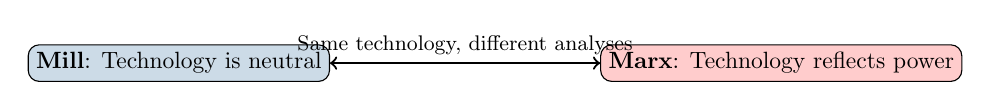
\begin{tikzpicture}[scale=0.85, transform shape]
  \node[draw, rounded corners, fill=primaryblue!20, minimum width=4cm] (mill) at (0,0) {\textbf{Mill}: Technology is neutral};
  \node[draw, rounded corners, fill=red!20, minimum width=4cm] (marx) at (9,0) {\textbf{Marx}: Technology reflects power};
  \draw[<->, thick] (mill) -- (marx) node[midway, above, font=\small] {Same technology, different analyses};
\end{tikzpicture}
\end{frame}

\begin{frame}{Quote: John Stuart Mill, \textit{On Liberty} (1859)}
\begin{exampleblock}{\faQuoteLeft\hspace{0.5em}John Stuart Mill, \textit{On Liberty}, Chapter 2}
\small
\textbf{Context:} Mill argues for absolute freedom of expression, claiming that silencing any opinion---even a false one---harms everyone.

\vspace{0.5em}
\textit{``If all mankind minus one were of one opinion, and only one person were of the contrary opinion, mankind would be \textbf{no more justified in silencing that one person}, than he, if he had the power, would be justified in silencing mankind.}

\vspace{0.3em}
\textit{But the \textbf{peculiar evil} of silencing the expression of an opinion is, that it is robbing the human race; posterity as well as the existing generation; those who dissent from the opinion, still more than those who hold it. If the opinion is right, they are deprived of the opportunity of exchanging error for truth: if wrong, they lose, what is almost as great a benefit, the clearer perception and livelier impression of truth, produced by its \textbf{collision with error}.''}
\end{exampleblock}

\vspace{0.2em}
\begin{block}{\faLightbulb\hspace{0.5em}The Assumption}
Mill assumes a ``marketplace of ideas'' where truth wins out. What conditions must hold for this to work?
\end{block}
\end{frame}

\begin{frame}{Marx's Counterargument}
\begin{argument}
  \item Those who \textbf{control the means of communication} control the dominant ideas in society.
  \item Under capitalism, the \textbf{ruling class} controls the means of communication.
  \item Therefore, ``free'' communication under capitalism primarily \textbf{serves ruling-class interests}.
  \item[\textbf{$\therefore$}] Genuine free communication requires \textbf{revolutionary change} in the ownership of communication technologies.
\end{argument}

\vspace{0.5em}
\discussion{Is Marx right that whoever \textbf{owns the technology} controls the message? Can you think of counterexamples?}

\vspace{0.3em}
\begin{alertblock}{The Challenge to Mill}
If the ``marketplace'' is rigged, can truth really win through ``free competition''?
\end{alertblock}
\end{frame}

\begin{frame}{Social Consequences of Distance Communication}
\begin{columns}
\begin{column}{0.48\textwidth}
\begin{block}{\faThumbsUp\hspace{0.3em}Benefits}
\begin{itemize}
  \item Coordination of \textbf{reform and labor movements}
  \item \textbf{Investigative journalism}
  \item \textbf{Scientific collaboration} across borders
  \item \textbf{Family connection} across vast distances
  \item Commercial efficiency
\end{itemize}
\end{block}
\end{column}

\begin{column}{0.48\textwidth}
\begin{alertblock}{\faThumbsDown\hspace{0.3em}Harms}
\begin{itemize}
  \item \textbf{Colonialism} and imperial coordination
  \item \textbf{Surveillance networks}
  \item Market manipulation and \textbf{speculation}
  \item Sensationalist \textbf{``yellow journalism''}
  \item \textbf{Cultural imperialism}
\end{itemize}
\end{alertblock}
\end{column}
\end{columns}

\vspace{0.5em}
\begin{exampleblock}{The Pattern Continues}
The telegraph and telephone that connected families also coordinated empires.
\end{exampleblock}
\end{frame}

% ====================
% REVOLUTION 4: MASS MEDIA (Slides 25-30)
% ====================

\begin{frame}{Revolution 4: The Rise of Radio and Television}
\begin{block}{Key Developments}
\begin{itemize}
  \item \textbf{Radio broadcasting} emerges in 1920s
  \item \textbf{Television} becomes dominant in 1950s
  \item \textbf{Structural shift}: Passive consumption, one-to-many broadcast model
  \item \textbf{Limited spectrum}: Corporate and state control
\end{itemize}
\end{block}

\vspace{0.3em}
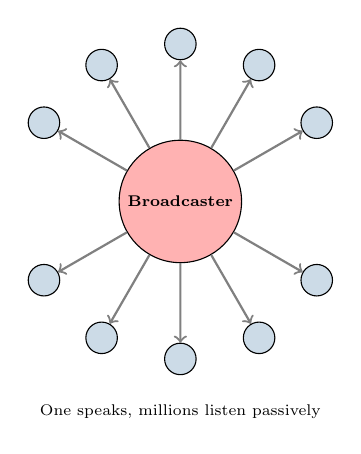
\begin{tikzpicture}[scale=0.8, transform shape]
  \node[draw, circle, fill=red!30, minimum size=1.2cm, font=\scriptsize\bfseries] (broadcast) at (0,0) {Broadcaster};
  \foreach \angle in {30,60,90,120,150,210,240,270,300,330} {
    \node[draw, circle, fill=primaryblue!20, minimum size=0.5cm, font=\tiny] (a\angle) at (\angle:2.5cm) {};
    \draw[->, thick, gray] (broadcast) -- (a\angle);
  }
  \node[below=0.3cm, font=\scriptsize] at (0,-2.8) {One speaks, millions listen passively};
\end{tikzpicture}

\vspace{0.2em}
\discussion{What makes radio and TV different from print? Think about who speaks and who listens.}
\end{frame}

\begin{frame}{Who Were Orwell and Arendt?}
\begin{columns}
\begin{column}{0.48\textwidth}
\begin{block}{George Orwell (1903--1950)}
\begin{itemize}
  \item Born Eric Arthur Blair in India
  \item British novelist, essayist, journalist
  \item Fought in \textbf{Spanish Civil War} (1936)
  \item Witnessed \textbf{Stalinist purges} firsthand
  \item Works: \textit{Animal Farm}, \textit{1984}
  \item Died of tuberculosis at 46
\end{itemize}
\end{block}
\end{column}

\begin{column}{0.48\textwidth}
\begin{exampleblock}{Hannah Arendt (1906--1975)}
\begin{itemize}
  \item German-Jewish philosopher
  \item \textbf{Fled Nazi Germany} (1933)
  \item Stateless refugee for 18 years
  \item Covered \textbf{Eichmann trial} (1961)
  \item Works: \textit{Origins of Totalitarianism}, \textit{Eichmann in Jerusalem}
  \item Coined ``\textbf{banality of evil}''
\end{itemize}
\end{exampleblock}
\end{column}
\end{columns}

\vspace{0.3em}
\begin{alertblock}{Why Their Perspective Matters}
Both \textbf{personally witnessed} the rise of totalitarianism. Their analyses come from \textbf{lived experience}, not just theory.
\end{alertblock}
\end{frame}

\begin{frame}{George Orwell's Warning}
\begin{block}{George Orwell (1903--1950)}
\begin{itemize}
  \item \textbf{\textit{1984}} (1949): Dystopian novel about totalitarian media control
  \item The \textbf{telescreen}: Watches you while you watch it
  \item \textbf{Propaganda slogans}: ``War is Peace, Freedom is Slavery, Ignorance is Strength''
  \item \textbf{Doublethink}: Holding two contradictory beliefs simultaneously
\end{itemize}
\end{block}

\vspace{0.3em}
\begin{alertblock}{Orwell's Central Concern}
A state \textbf{monopoly on information} makes \textbf{reality itself malleable}. If the Party controls all records, truth becomes whatever the Party says it is.
\end{alertblock}

\vspace{0.3em}
\begin{exampleblock}{Historical Context}
Orwell wrote \textit{1984} in 1948, having witnessed the rise of Nazi Germany and Stalinist Russia---both masters of propaganda.
\end{exampleblock}
\end{frame}

\begin{frame}{Quote: George Orwell, \textit{1984}}
\begin{exampleblock}{\faQuoteLeft\hspace{0.5em}George Orwell, \textit{Nineteen Eighty-Four}, Book 1, Chapter 7}
\small
\textbf{Context:} Winston Smith works at the Ministry of Truth, rewriting historical records. Here he reflects on the Party's ultimate demand---not just obedience, but the surrender of one's own perceptions.

\vspace{0.5em}
\textit{``The Party told you to \textbf{reject the evidence of your eyes and ears}. It was their final, most essential command. His heart sank as he thought of the enormous power arrayed against him, the ease with which any Party intellectual would overthrow him in debate, the subtle arguments which he would not be able to understand, much less answer.}

\vspace{0.3em}
\textit{And yet he was in the right! They were wrong and he was right. \textbf{The obvious, the silly, and the true had got to be defended. Truisms are true, hold on to that!}''}
\end{exampleblock}

\vspace{0.2em}
\begin{block}{\faLightbulb\hspace{0.5em}The Ultimate Goal}
Not just to make you believe lies, but to \textbf{destroy your capacity to distinguish truth from falsehood}.
\end{block}
\end{frame}

\begin{frame}{Hannah Arendt on Mass Society}
\begin{block}{Hannah Arendt (1906--1975)}
\begin{itemize}
  \item \textbf{\textit{The Origins of Totalitarianism}} (1951)
  \item Analyzed how totalitarian movements gained power
  \item Key insight: The precondition wasn't \textbf{ideology} but \textbf{loneliness}
  \item Breakdown of social bonds leaves individuals vulnerable
\end{itemize}
\end{block}

\vspace{0.3em}
\begin{exampleblock}{\faQuoteLeft\hspace{0.5em}Hannah Arendt, \textit{The Origins of Totalitarianism}, Chapter 13}
\small
\textit{``What prepares men for totalitarian domination in the non-totalitarian world is the fact that \textbf{loneliness}, once a borderline experience usually suffered in certain marginal social conditions like old age, has become an \textbf{everyday experience} of the ever-growing masses of our century.''}
\end{exampleblock}

\vspace{0.2em}
\begin{alertblock}{\faLightbulb\hspace{0.5em}The Insight}
Mass media doesn't just spread propaganda---it helps create the \textbf{atomized, isolated individuals} who crave belonging so desperately that they'll join movements promising meaning.
\end{alertblock}
\end{frame}

\begin{frame}{Arendt's Analysis of Propaganda}
\begin{argument}
  \item Mass society produces \textbf{isolated, ``atomized'' individuals} who feel superfluous.
  \item Lonely individuals \textbf{crave coherent explanations} that give their lives meaning.
  \item Mass media can deliver such explanations \textbf{directly to millions simultaneously}.
  \item Totalitarian movements \textbf{exploit this} by offering all-encompassing ideologies.
  \item[\textbf{$\therefore$}] Mass media combined with mass loneliness creates conditions \textbf{favorable to totalitarianism}.
\end{argument}

\vspace{0.5em}
\discussion{Does social media make us \textbf{more or less lonely} than broadcast media did?}

\vspace{0.3em}
\begin{alertblock}{The Question for Us}
If Arendt is right, then the problem isn't just \textit{what} media says, but \textit{what it does} to social bonds.
\end{alertblock}
\end{frame}

\begin{frame}{Social Consequences of Mass Media}
\begin{columns}
\begin{column}{0.48\textwidth}
\begin{block}{\faThumbsUp\hspace{0.3em}Benefits}
\begin{itemize}
  \item \textbf{Mass education}
  \item \textbf{Shared cultural experiences}
  \item Exposure to \textbf{diversity}
  \item \textbf{Rapid news dissemination}
  \item \textbf{Public health campaigns}
  \item Civil rights coverage
\end{itemize}
\end{block}
\end{column}

\begin{column}{0.48\textwidth}
\begin{alertblock}{\faThumbsDown\hspace{0.3em}Harms}
\begin{itemize}
  \item \textbf{Propaganda effectiveness}
  \item ``Manufacturing consent''
  \item \textbf{Advertising and consumerism}
  \item \textbf{Political manipulation}
  \item Homogenization of culture
  \item \textbf{Passivity}: ``The Lonely Crowd''
\end{itemize}
\end{alertblock}
\end{column}
\end{columns}

\vspace{0.5em}
\begin{exampleblock}{The Paradox}
The same broadcast that showed the Civil Rights Movement to the nation also enabled unprecedented propaganda.
\end{exampleblock}
\end{frame}

% ====================
% REVOLUTION 5: THE WEB (Slides 31-35)
% ====================

\begin{frame}{Revolution 5: Web 1.0---The Read-Only Web (1990s)}
\begin{block}{Key Developments}
\begin{itemize}
  \item \textbf{Tim Berners-Lee} invents the World Wide Web (1989--1991)
  \item \textbf{Static pages}, hyperlinks, information retrieval
  \item Early \textbf{utopian visions}: Free information, democratization, disintermediation
  \item ``\textbf{Information wants to be free}''---Stewart Brand
\end{itemize}
\end{block}

\vspace{0.3em}
\begin{exampleblock}{The Promise}
The early web was hailed as the \textbf{great equalizer}---anyone could publish, anyone could access.
\end{exampleblock}

\vspace{0.3em}
\discussion{The early web was hailed as the great equalizer. How did that work out?}
\end{frame}

\begin{frame}{Web 2.0---The Participatory Web (2000s)}
\begin{block}{Key Developments}
\begin{itemize}
  \item \textbf{Social media}, user-generated content
  \item \textbf{Platforms}: Facebook, YouTube, Twitter/X, Wikipedia, TikTok
  \item \textbf{Promise}: Everyone becomes a creator, not just a consumer
  \item \textbf{Reality}: The attention economy and algorithmic curation
\end{itemize}
\end{block}

\vspace{0.3em}
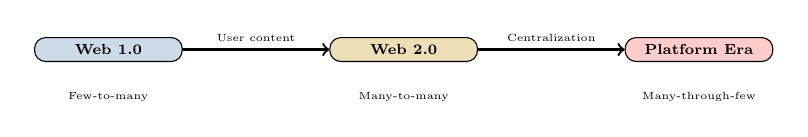
\begin{tikzpicture}[scale=0.75, transform shape]
  \node[draw, rounded corners, fill=primaryblue!20, minimum width=2.5cm, font=\scriptsize\bfseries] (web1) at (0,0) {Web 1.0};
  \node[draw, rounded corners, fill=accentgold!30, minimum width=2.5cm, font=\scriptsize\bfseries] (web2) at (5,0) {Web 2.0};
  \node[draw, rounded corners, fill=red!20, minimum width=2.5cm, font=\scriptsize\bfseries] (platform) at (10,0) {Platform Era};
  \draw[->, thick] (web1) -- (web2) node[midway, above, font=\tiny] {User content};
  \draw[->, thick] (web2) -- (platform) node[midway, above, font=\tiny] {Centralization};
  \node[below, font=\tiny, text width=2.5cm, align=center] at (0,-0.6) {Few-to-many};
  \node[below, font=\tiny, text width=2.5cm, align=center] at (5,-0.6) {Many-to-many};
  \node[below, font=\tiny, text width=2.5cm, align=center] at (10,-0.6) {Many-through-few};
\end{tikzpicture}

\vspace{0.3em}
\begin{alertblock}{New Intermediaries}
Platform companies become the new \textbf{gatekeepers}---and they're driven by advertising revenue.
\end{alertblock}
\end{frame}

\begin{frame}{Web 3.0?---Contested Futures}
\begin{block}{Competing Visions}
\begin{itemize}
  \item \textbf{Semantic web / AI integration}: Machines understand meaning
  \item \textbf{Blockchain and decentralization}: Removing intermediaries (?)
  \item \textbf{Virtual and augmented reality}: Immersive digital worlds
  \item \textbf{Artificial intelligence}: ChatGPT, image generation, and beyond
\end{itemize}
\end{block}

\vspace{0.3em}
\begin{columns}
\begin{column}{0.48\textwidth}
\begin{exampleblock}{Utopian Vision}
\begin{itemize}
  \item Digital liberation
  \item Democratized AI tools
  \item Decentralized power
\end{itemize}
\end{exampleblock}
\end{column}

\begin{column}{0.48\textwidth}
\begin{alertblock}{Dystopian Vision}
\begin{itemize}
  \item Surveillance capitalism
  \item Deepfakes and misinformation
  \item Algorithmic control
\end{itemize}
\end{alertblock}
\end{column}
\end{columns}

\vspace{0.3em}
\discussion{What would a truly \textbf{decentralized} internet look like? Is it even possible?}
\end{frame}

\begin{frame}{Current Debates}
\begin{table}
\centering
\small
\begin{tabular}{@{}p{4.5cm}p{4.5cm}p{4.5cm}@{}}
\toprule
\textbf{Debate} & \textbf{Position A} & \textbf{Position B} \\
\midrule
Free speech vs. moderation & Maximize expression & Prevent harm \\
Privacy vs. convenience & Protect personal data & Enable services \\
Platforms as publishers? & Yes, they curate & No, they're neutral \\
Algorithmic amplification & Personalization helps & Manipulation harms \\
AI benefits vs. risks & Productivity gains & Job loss, misuse \\
\bottomrule
\end{tabular}
\end{table}

\vspace{0.5em}
\discussion{Which of these debates do you find most pressing? Why?}

\vspace{0.3em}
\begin{alertblock}{The Recurring Question}
Who decides? And on what basis?
\end{alertblock}
\end{frame}

% ====================
% CONCLUSION (Slides 35-36)
% ====================

\begin{frame}{Patterns Across the Revolutions}
\begin{table}
\centering
\scriptsize
\begin{tabular}{@{}llllp{2.8cm}@{}}
\toprule
\textbf{Revolution} & \textbf{Technology} & \textbf{Optimist} & \textbf{Pessimist} & \textbf{Core Tension} \\
\midrule
Writing & Alphabet, scrolls & Theuth & Socrates & Memory vs. Reminding \\
Printing & Movable type & Luther & Erasmus & Revolution vs. Reform \\
Distance & Telegraph, phone & Mill & Marx & Free market vs. Ownership \\
Mass Media & Radio, TV & --- & Orwell, Arendt & Information vs. Control \\
The Web & Internet, platforms & Early utopians & (Us?) & Liberation vs. Surveillance \\
\bottomrule
\end{tabular}
\end{table}

\vspace{0.3em}
\begin{block}{Recurring Themes}
\begin{itemize}
  \item Each revolution promised \textbf{liberation and democratization}
  \item Each enabled \textbf{new forms of control and manipulation}
  \item The optimists and pessimists were \textbf{both partially right}
  \item The question is always: \textbf{Who controls the technology, and for what ends?}
\end{itemize}
\end{block}
\end{frame}

\begin{frame}{Looking Ahead}
\begin{block}{Why History Matters for IT Ethics}
\begin{itemize}
  \item We are \textbf{not the first} to face these questions
  \item The ``debates'' we're having are \textbf{ancient}
  \item Understanding patterns helps us \textbf{think more clearly} about the present
\end{itemize}
\end{block}

\vspace{0.3em}
\begin{exampleblock}{Course Roadmap}
From \textbf{History} $\rightarrow$ \textbf{Ethical Frameworks} $\rightarrow$ \textbf{Contemporary Issues}
\end{exampleblock}

\vspace{0.3em}
\begin{alertblock}{\faQuoteLeft\hspace{0.5em}Final Thought}
\textit{``Those who cannot remember the past are condemned to repeat it.''}\\
\hfill---George Santayana, \textit{The Life of Reason} (1905)
\end{alertblock}

\vspace{0.3em}
\discussion{What responsibilities do we have as participants in the current IT revolution?}
\end{frame}

\end{document}